\documentclass{article}

\usepackage{amsmath,amssymb}
\usepackage{tikz}
\usetikzlibrary{er,positioning}
\usepackage{pgfplots}
\usepackage{xcolor}
\usepackage[left=2.1cm,right=3.1cm,bottom=3cm,footskip=0.75cm,headsep=0.5cm]{geometry}
\usepackage{enumerate}
\usepackage{enumitem}
\usepackage{marvosym}
\usepackage{tabularx}
\usepackage{parskip}
\usepackage{longtable}

\usepackage{listings}
\definecolor{lightlightgray}{rgb}{0.95,0.95,0.95}
\definecolor{lila}{rgb}{0.8,0,0.8}
\definecolor{mygray}{rgb}{0.5,0.5,0.5}
\definecolor{mygreen}{rgb}{0,0.8,0.26}
\lstdefinestyle{sql} {language=sql}
\lstset{language=sql,
	basicstyle=\ttfamily,
	keywordstyle=\color{lila},
	commentstyle=\color{lightgray},
	stringstyle=\color{mygreen}\ttfamily,
	backgroundcolor=\color{white},
	showstringspaces=false,
	numbers=left,
	numbersep=10pt,
	numberstyle=\color{mygray}\ttfamily,
	identifierstyle=\color{blue},
	xleftmargin=.1\textwidth, 
	%xrightmargin=.1\textwidth,
	escapechar=§,
}

\usepackage[utf8]{inputenc}

\renewcommand*{\arraystretch}{1.4}

\newcolumntype{L}[1]{>{\raggedright\arraybackslash}p{#1}}
\newcolumntype{R}[1]{>{\raggedleft\arraybackslash}p{#1}}
\newcolumntype{C}[1]{>{\centering\let\newline\\\arraybackslash\hspace{0pt}}m{#1}}

\newcommand{\E}{\mathbb{E}}
\DeclareMathOperator{\rk}{rk}
\DeclareMathOperator{\Var}{Var}
\DeclareMathOperator{\Cov}{Cov}

\def\ojoin{\setbox0=\hbox{$\bowtie$}%
	\rule[-.02ex]{.25em}{.4pt}\llap{\rule[\ht0]{.25em}{.4pt}}}
\def\leftouterjoin{\mathbin{\ojoin\mkern-5.8mu\bowtie}}
\def\rightouterjoin{\mathbin{\bowtie\mkern-5.8mu\ojoin}}
\def\fullouterjoin{\mathbin{\ojoin\mkern-5.8mu\bowtie\mkern-5.8mu\ojoin}}

\title{\textbf{Datenbanken, Hands-on 1}}
\author{\textsc{Henry Haustein}}
\date{}

\begin{document}
	\maketitle
	
	Eine Vorbemerkung: Ich weiß nicht, inwieweit diese Aufgaben richtig gelöst sind, ich würde mich also freuen, wenn jemand mit einem anderen Ansatz meine Zahlen mal überprüft und es als Kommentar postet.
	
	\section*{Aufgabe 1}
	Eine mögliche SQL-Abfrage ist z.B.
	\begin{lstlisting}[style=sql]
SELECT area, count(area) AS anzahl 
FROM artist 
WHERE begin_date_year < 1850 
GROUP BY area HAVING anzahl > 10 
ORDER BY anzahl DESC;
	\end{lstlisting}
	Dieser liefert eine Liste mit den Area-IDs und deren Vorkommen in der Tabelle \texttt{artist}. Zusätzlich filtern wir noch nach Geburtsdatum vor 1850 (\texttt{WHERE\ begin\_date\_year < 1850}) und es müssen mehr als 10 Vorkommen in der Tabelle sein (\texttt{HAVING anzahl > 10}). Das HAVING-Statement ist nötig, weil so etwas wie \texttt{WHERE anzahl > 10} einen Fehler erzeugt.
	
	Will man noch den Namen der entsprechenden Regionen angezeigt bekommen, ist die SQL-Abfrage etwas aufwendiger:
	\begin{lstlisting}[style=sql]
SELECT artist.area, area.name, count(artist.area) AS anzahl 
FROM artist, area 
WHERE artist.begin_date_year < 1850 AND artist.area = area.id 
GROUP BY artist.area HAVING count(artist.area) > 10 
ORDER BY anzahl DESC;
	\end{lstlisting}
	Diese liefert die folgende Tabelle:
	\begin{center}
		\begin{longtable}{l|l|l}
			\textbf{artist.area} & \textbf{area.name} & \textbf{anzahl} \\ \hline
			81 & Germany & 1543 \\ \hline
			73 & France & 1169 \\ \hline
			105 & Italy & 1049 \\ \hline
			221 & United Kingdom & 766 \\ \hline
			14 & Austria & 355 \\ \hline
			222 & United States & 344 \\ \hline
			194 & Spain & 270 \\ \hline
			176 & Russia & 191 \\ \hline
			432 & England & 181 \\ \hline
			56 & Czech Republic & 156 \\ \hline
			57 & Denmark & 151 \\ \hline
			202 & Sweden & 148 \\ \hline
			21 & Belgium & 130 \\ \hline
			150 & Netherlands & 118 \\ \hline
			214 & Turkey & 114 \\ \hline
			170 & Poland & 91 \\ \hline
			72 & Finland & 70 \\ \hline
			160 & Norway & 70 \\ \hline
			97 & Hungary & 64 \\ \hline
			103 & Ireland & 57 \\ \hline
			203 & Switzerland & 55 \\ \hline
			434 & Scotland & 39 \\ \hline
			171 & Portugal & 38 \\ \hline
			435 & Wales & 35 \\ \hline
			44 & China & 34 \\ \hline
			107 & Japan & 33 \\ \hline
			1794 & Flanders & 29 \\ \hline
			30 & Brazil & 23 \\ \hline
			67 & Estonia & 22 \\ \hline
			38 & Canada & 19 \\ \hline
			4434 & Paris & 19 \\ \hline
			99 & India & 18 \\ \hline
			117 & Latvia & 17 \\ \hline
			84 & Greece & 16 \\ \hline
			138 & Mexico & 15 \\ \hline
			175 & Romania & 12 \\ \hline
			219 & Ukraine & 11 \\ \hline
			1178 & London & 11
		\end{longtable}
	\end{center}
	Mit insgesamt 38 Einträgen. Hier sieht man auch, dass in der Aufgabenstellung mit \textit{Länder} eigentlich die Areas gemeint sind. Ich habe extra noch mal nachgefragt, \textit{Länder} wie London sollen mitgezählt werden.

	\section*{Aufgabe 2}
	Wir brauchen die ID der Gruppe \textit{Arcade Fire}, das ist das passende SQL-Statement dazu:
	\begin{lstlisting}[style=sql]
SELECT * FROM artist WHERE name = "Arcade Fire";
	\end{lstlisting}
	Das liefert uns die ID 164813. Damit können wir uns anzeigen lassen, mit wem die Gruppe zusammengearbeitet hat:
	\begin{lstlisting}[style=sql]
SELECT * FROM artist_credit_name WHERE artist = 164813;
	\end{lstlisting}
	\begin{center}
		\begin{tabular}{l|l|l|l}
			\textbf{artist\_credit} & \textbf{position} & \textbf{artist} & \textbf{name} \\ \hline
			164813 & 0 & 164813 & Arcade Fire \\ \hline
			822784 & 0 & 164813 & Arcade Fire \\ \hline
			823326 & 1 & 164813 & Arcade Fire \\ \hline
			867032 & 0 & 164813 & Arcade Fire \\ \hline
			973655 & 1 & 164813 & Arcade Fire \\ \hline
			997531 & 1 & 164813 & Arcade Fire \\ \hline
			1317313 & 1 & 164813 & Arcade Fire \\ \hline
			1230340 & 0 & 164813 & The Reflektors \\ \hline
			1540340 & 0 & 164813 & Arcade Fire \\ \hline
			1648422 & 1 & 164813 & Arcade Fire \\ \hline
			2028174 & 2 & 164813 & Arcade Fire \\ \hline
			1779951 & 0 & 164813 & Arcade Fire \\ \hline
			1779952 & 0 & 164813 & Arcade Fire \\ \hline
			1875665 & 0 & 164813 & Arcade Fire \\ \hline
			2295985 & 0 & 164813 & Arcade Fire
		\end{tabular}
	\end{center}
	Jetzt suchen wir uns die richtigen IDs für die in der Aufgabenstellung vorgegebenen Formate raus. Die Bedingung \texttt{name LIKE "\%vinyl\%"} ist dann erfüllt, wenn \texttt{name} das Wort \textit{vinyl} an irgendeiner Stelle enthält (die \% sind so eine Art Platzhalter für jede Buchstabenkombination).
	\begin{lstlisting}[style=sql]
SELECT * 
FROM medium_format 
WHERE name LIKE "%vinyl%" AND name != "VinylDisc";
	\end{lstlisting}
	Das liefert uns
	\begin{center}
		\begin{longtable}{l|l|L{9cm}}
			\textbf{id} & \textbf{name} & \textbf{description} \\ \hline
			29 & 7" Vinyl & | \\ \hline
			30 & 10" Vinyl & | \\ \hline
			31 & 12" Vinyl & | \\ \hline
			7 & Vinyl & | \\ \hline
			80 & VinylDisc (DVD side) & The DVD side of a vinyl + DVD VinylDisc. The vinyl side should be added as a separate medium. \\ \hline
			81 & VinylDisc (Vinyl side) & The vinyl side of a VinylDisc. The CD or DVD side should be added as a separate medium. \\ \hline
			82 & VinylDisc (CD side) & The CD side of a vinyl + CD VinylDisc. The vinyl side should be added as a separate medium.
		\end{longtable}
	\end{center}
	Damit können wir alle Releases finden, die das richtige Format haben. Besonders nützlich erweist sich hier die WHERE-IN-Klausel, mit der wir überprüfen können, ob ein Attribut einen Wert aus einer Liste annimmt. Diese Liste liefern mit einer Subquery.
	\begin{lstlisting}[style=sql]
SELECT * 
FROM medium 
WHERE format IN 
	(SELECT id FROM medium_format 
	WHERE name LIKE "%vinyl%" AND name != "VinylDisc");
	\end{lstlisting}
	Das liefert 352703 Ergebnisse, unter anderem
	\begin{center}
		\begin{tabular}{l|l|l|l|l}
			\textbf{id} & \textbf{release} & \textbf{position} & \textbf{format} & \textbf{name} \\ \hline
			384122 & 384122 & 1 & 31 & | \\ \hline
			369088 & 369088 & 1 & 31 & | \\ \hline
			948451 & 948451 & 1 & 31 & | \\ \hline
			600903 & 600903 & 1 & 31 & | \\ \hline
			47158 & 47158 & 1 & 31 & | \\ \hline
			588082 & 588082 & 1 & 31 & | \\ \hline
			26221 & 26221 & 1 & 31 & | \\ \hline
			709966 & 709966 & 1 & 31 & | \\ \hline
			709967 & 709967 & 1 & 31 & | \\ \hline
			593289 & 593289 & 1 & 7 & |
		\end{tabular}
	\end{center}
	Endlich können wir die finale SQL-Abfrage zusammensetzen: Dazu schauen wir in der release-Tabelle nach den Releases im richtigen Format und dem richtigen Künstler. Duplikate im Namen filtern wir mit dem GROUP-BY-Statement
	\begin{lstlisting}[style=sql]
SELECT * 
FROM release 
WHERE artist_credit IN 
	(SELECT artist_credit 
	FROM artist_credit_name 
	WHERE artist = 164813)
AND id IN 
	(SELECT id FROM medium WHERE format IN 
		(SELECT id 
		FROM medium_format 
		WHERE name LIKE "%vinyl%" AND name != "VinylDisc")
	)
GROUP BY name;
	\end{lstlisting}
	Das liefert uns folgende Tabelle mit 17 Einträgen.
	\begin{center}
		\begin{tabular}{l|L{3cm}|l|l|l|l}
			\textbf{id} & \textbf{name} & \textbf{artist\_credit} & \textbf{status} & \textbf{language} & \textbf{comment} \\ \hline
			2011803 & Alting Nu & 164813 & 1 & 120 & Danish limited version \\ \hline
			1304715 & Arcade Fire & 164813 & 1 & 120 & remaster \\ \hline
			2389021 & Baby Mine & 164813 & 1 & 120 & | \\ \hline
			57460 & Cold Wind / Brazil & 164813 & 1 & 120 & | \\ \hline
			2007060 & Everything Now & 164813 & 1 & 120 & Day version \\ \hline
			252852 & Funeral & 164813 & 1 & 120 & | \\ \hline
			287958 & Intervention & 164813 & 1 & 120 & | \\ \hline
			252655 & Keep the Car Running / Broken Window & 164813 & 1 & 120 & | \\ \hline
			820844 & Neon Bible & 164813 & 1 & 120 & | \\ \hline
			301944 & No Cars Go & 164813 & 1 & 120 & | \\ \hline
			312976 & Poupée de cire, poupée de son / No Love Lost & 997531 & 1 & 120 & | \\ \hline
			227251 & Rebellion (Lies) & 164813 & 1 & 120 & | \\ \hline
			1345908 & Reflektor & 164813 & 1 & 120 & | \\ \hline
			2330208 & The Reflektor Tapes & 164813 & 1 & 120 & | \\ \hline
			730810 & The Suburbs & 164813 & 1 & 120 & | \\ \hline
			697791 & The Suburbs / Month of May & 164813 & 1 & 120 & | \\ \hline
			2138539 & $\langle\text{Hindi-Text}\rangle$ & 164813 & 1 & 120 & Hindi limited version
		\end{tabular}
	\end{center}

	\section*{Aufgabe 3}
	Die folgende SQL-Abfrage liefert uns direkt das Ergebnis:
	\begin{lstlisting}[style=sql]
SELECT count(*) 
FROM release_info 
WHERE date_year >= 1980 AND date_year < 1990;
	\end{lstlisting}
	Es sind 139614 Releases.
	
	\section*{Aufgabe 4}
	Zuerst brauchen wir wieder die ID von \textit{Ariana Grande}:
	\begin{lstlisting}[style=sql]
SELECT * FROM artist WHERE name = "Ariana Grande";
	\end{lstlisting}
	Sie hat die ID 823336.
	
	Damit können wir nach Mitproduzenten suchen und auch gleich zählen lassen:
	\begin{lstlisting}[style=sql]
SELECT count(*) FROM artist_credit_name WHERE artist = 823336;
	\end{lstlisting}
	Es sind 173.
	
	\section*{Aufgabe 5}
	Wieder suchen wir uns die ID der \textit{The Beatles}:
	\begin{lstlisting}[style=sql]
SELECT * FROM artist WHERE name = "The Beatles";
	\end{lstlisting}
	und erhalten 303.
	
	Damit können wir die \texttt{artist-alias}-Tabelle fragen:
	\begin{lstlisting}[style=sql]
SELECT * FROM artist_alias WHERE artist = 303;
	\end{lstlisting}
	und erhalten
	\begin{center}
		\begin{longtable}{l|l|l}
			\textbf{id} & \textbf{artist} & \textbf{name} \\ \hline
			179051 & 303 & B \\ \hline
			106844 & 303 & $\langle\text{nicht darstellbar}\rangle$ \\ \hline
			10389 & 303 & fab four \\ \hline
			117401 & 303 & $\langle\text{nicht darstellbar}\rangle$ \\ \hline
			165662 & 303 & The Beatles \\ \hline
			1126 & 303 & Beetles \\ \hline
			179055 & 303 & Be \\ \hline
			179056 & 303 & Beat \\ \hline
			130 & 303 & Beatles \\ \hline
			184586 & 303 & The Savage Young Beatles \\ \hline
			241307 & 303 & Les Beatles \\ \hline
			76594 & 303 & $\langle\text{nicht darstellbar}\rangle$ \\ \hline
			106841 & 303 & Los Beatles \\ \hline
			263503 & 303 & $\langle\text{nicht darstellbar}\rangle$ \\ \hline
			263502 & 303 & $\langle\text{nicht darstellbar}\rangle$ \\ \hline
			263504 & 303 & $\langle\text{nicht darstellbar}\rangle$ \\ \hline
			263506 & 303 & $\langle\text{nicht darstellbar}\rangle$ \\ \hline
			263507 & 303 & $\langle\text{nicht darstellbar}\rangle$ \\ \hline
			263508 & 303 & $\langle\text{nicht darstellbar}\rangle$ \\ \hline
			76592 & 303 & $\langle\text{nicht darstellbar}\rangle$ \\ \hline
			263509 & 303 & $\langle\text{nicht darstellbar}\rangle$ \\ \hline
			263510 & 303 & Bítlarnir \\ \hline
			263511 & 303 & $\langle\text{nicht darstellbar}\rangle$ \\ \hline
			263512 & 303 & $\langle\text{nicht darstellbar}\rangle$ \\ \hline
			263513 & 303 & $\langle\text{nicht darstellbar}\rangle$ \\ \hline
			263514 & 303 & $\langle\text{nicht darstellbar}\rangle$ \\ \hline
			263515 & 303 & $\langle\text{nicht darstellbar}\rangle$ \\ \hline
			263516 & 303 & $\langle\text{nicht darstellbar}\rangle$ \\ \hline
			263517 & 303 & $\langle\text{nicht darstellbar}\rangle$ \\ \hline
			263518 & 303 & $\langle\text{nicht darstellbar}\rangle$ \\ \hline
			263519 & 303 & $\langle\text{nicht darstellbar}\rangle$ \\ \hline
			263520 & 303 & Die Beatles \\ \hline
			263521 & 303 & I Beatles \\ \hline
			263523 & 303 & The Silver Beatles \\ \hline
			115264 & 303 & $\langle\text{nicht darstellbar}\rangle$
		\end{longtable}
	\end{center}
	Da ich viele dieser Sonderzeichen nicht darstellen kann, gibt es hier ein Bild:
	\begin{center}
		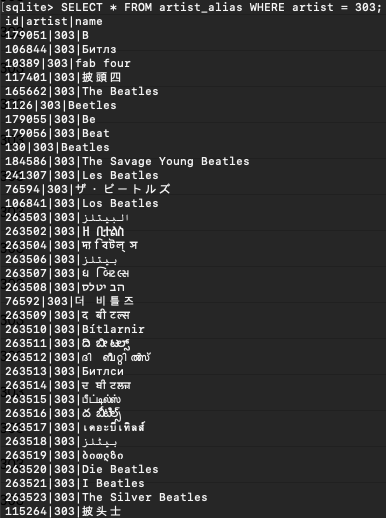
\includegraphics[width=0.50\textwidth]{aufgabe5}
	\end{center}
	Wie das mit dem WITH-Statement funktioniert, habe ich bisher nicht rausgefunden, deswegen habe ich die einzelnen Namen händisch zusammengefügt und kam am Ende auf eine Länge von 354 Zeichen.
	
\end{document}